% This is part of Un soupçon de mathématique sans être agressif pour autant
% Copyright (c) 2015
%   Laurent Claessens
% See the file fdl-1.3.txt for copying conditions.

\begin{exercice}\label{exo2smath-0178}

    Estelle dit que les deux dessins suivants sont des parallélogrammes :
    \begin{center}
    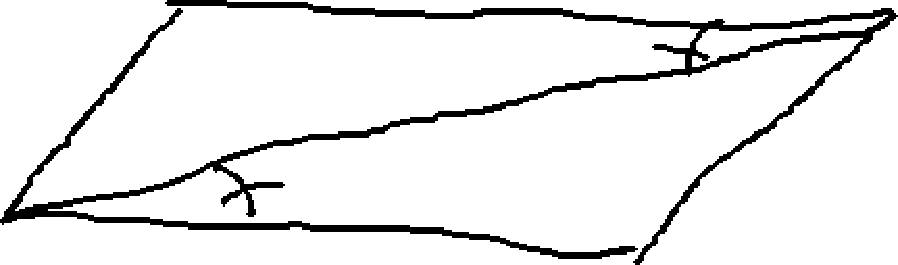
\includegraphics[width=\linewidth]{codage_parall1.pdf}      % Ce graphique est également utilisé dans exo2smath-0325
    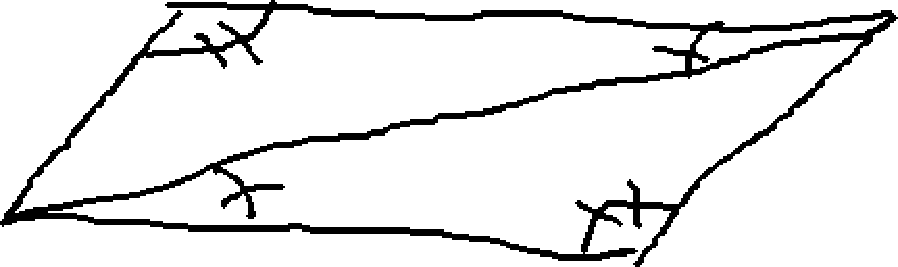
\includegraphics[width=\linewidth]{codage_parall2.pdf}
    \end{center}
    Mais Alisée soutient que seulement le second est un parallélogramme. Ce à quoi Estelle répond que le second est en réalité un losange.

    Peut-on démêler le vrai du faux dans tout cela ?

\corrref{2smath-0178}
\end{exercice}
